\section{Основы линейной и нелинейной оптики.}

\subsection{Материальное уравнение линейной среды.}
\hspace*{2mm}В основе взаимодействия света со средой лежит элементарный
процесс возбуждения атома или молекулы вещества световым полем и последующего переизлучения света возбужденной частицей. Характер этого взаимодействия зависит от соотношения между величиной напряженности поля световой волны Е и характерной напряженностью внутриатомного поля $E_{atom}$, определяющего силы связи оптических электронов (т.е. внешних, наиболее слабо связанных электронов) с ядром атома вещества.
\\
\hspace*{2mm}
Для атома водорода это поле составляет $ E_{atom} = e/(4\pi\epsilon_{0}r_{h}^2) = 5\cdot10^{11} $В/м, для более тяжелых атомов $ E_{atom} = 10^{10} \dots 10^{11} $ В/м. Оценка поля Е световой волны в случае нелазерных источников свет дает величину $E \le 10^3$ В/м, т.е. $E<<E_{atom} $. При этом условии отклик атомного осциллятора на внешнее воздействие будет иметь линейный характер, а зависимость поляризованности Р = Р(Е) в случае изотропной среды может быть представлена в виде:
\begin{equation}\label{1:liner}
P(E) = \chi^{(1)}E
\end{equation}

где $ \chi^{(1)}$ – линейная восприимчивость среды, являющаяся безразмерной величиной и зависящая только от свойств среды.
Материальное уравнение ($\ref{1:liner}$) является одним из соотношений, на которых базируется линейная оптика.  Оно справедливо только при условии $E << E_{atom} $, а при невыполнении этого условия является лишь некоторым приближением.В мощных лазерных пучках можно получить напряженности уже сравнимые с $E_{atom} $. В случае когда поле Е, оставаясь меньше $E_{atom} $, приближается к нему по величине, поляризованность среды Р = Р(Е) перестает быть линейной функцией поля Е, и в этом случае материальное уравнение ($\ref{1:liner}$) должно быть заменено на другое.

\subsection{Материальное уравнение нелинейной среды.} 
\hspace*{2mm}Теория нелинейно-оптических явлений строится на основе материальных уравнений и уравнений
Максвелла. Уравнения Максвелла для диэлектрической нейтральной немагнитной среды имеют вид
\begin{equation}\label{1:maxvel}
rot\vec{E} = - \frac{ 1 }{ c}\frac{\partial \vec{H} }{\partial t}
\hspace{20mm}
rot\vec{H} =  \frac{ 1 }{ c}\frac{\partial \vec{D} }{\partial t}
\hspace{20mm}
div\vec{H} = 0
\end{equation}
где $ \vec{D} = \vec{E} + 4\pi \vec{P}$. Из уравнений Максвелла вытекает волновое уравнение
\begin{equation}\label{1:rot_maxvel}
rot(rot\vec{E}) + \frac{ 1 }{ c^2 }\frac{\partial^2 \vec{E} }{\partial t^2} = - \frac{ 4\pi }{ c^2 }\frac{\partial^2 \vec{P} }{\partial t^2}
\end{equation}
которе в случае изотропной среды принимает вид
\begin{equation}\label{1:wave_eq}
\Delta\vec{E} - \frac{ 1 }{ c^2 }\frac{\partial^2 \vec{E} }{\partial t^2} =  \frac{ 4\pi }{ c^2 }\frac{\partial^2 \vec{P} }{\partial t^2}
\end{equation}
где $\vec{E}$ - напряженность электрического поля, а $\vec{P}$ - поляризация среды. Поляризация среды возникает под действием падающий световой волны и описывается материальным уравнением $\vec{P} = \vec{P}(\vec{E})$.
В анизотропном случае $\vec{P}(\vec{E})$ являеться тензорный величиной и может быть представлена в виде:
\begin{equation}\label{1:p_1}
P(E) = \chi^{(1)}E + \chi^{(2)}E^2 \chi^{(3)}E^3\dots
\end{equation}
Коэффициенты $\chi^{m}, m \ge 2$ при членах разложения называются нелинейными восприимчивостями m-го порядка и являются уже размерными величинами. При этом соответствующая величина $\chi^{m}$ пропорциональна концентрации атомов (молекул) в веществе и m-ой степени параметра. Это означает, что отклик среды на действие внешнего светового поля перестает быть линейным.  С математической точки зрения именно это обстоятельство (нелинейность материального уравнения) является причиной нарушения принципа суперпозиции для световых волн в нелинейной среде. Из уравнений (\ref{1:rot_maxvel}), (\ref{1:wave_eq}) и (\ref{1:p_1}) непосредственно вытекает возможность генерации оптических гармоник и других нелинейно-оптических эффектов.  Надо отметить, что среды, в которых достаточно учитывать только первых два члена в уравнении ($\ref{1:wave_eq}$), называют квадратично-нелинейными средами, а среды с тремя первыми членами - кубически-нелинейными. 
\subsection{Нелинейная поляризация.} 
Часть поляризации среды, нелинейно зависящая от напряженности светового поля, называется нелинейной поляризацией.
Выделяя в поляризации среды линейную и нелинейную компоненты, можно
записать:
\begin{equation}\label{1:p_non_liner}
\vec{P} = \vec{P}_{liner} + \vec{P}_{nonliner}
\end{equation}
подставив уравнение  (\ref{1:p_non_liner}) в  (\ref{1:rot_maxvel}) получим волновое уравнение для анизотропной среды и нелинейной изотропной среды:
\begin{equation}\label{1:wave_eq2}
\Delta\vec{E} - \frac{ 1 }{ c^2 }\frac{\partial^2 \vec{E} }{\partial t^2} - \frac{ 4\pi }{ c^2 }\frac{\partial^2 \vec{P}_{liner}}{\partial t^2} =  \frac{ 4\pi }{ c^2 }\frac{\partial^2 \vec{P} _{nonliner}}{\partial t^2}
\end{equation}
 Нелинейная поляризация среды является источником новых спектральных компонент поля
(оптических гармоник, комбинационных частот и т. п.). Материальное уравнение вида  (\ref{1:wave_eq}), описывает изотропную нелинейную среду с безынерционным локальным откликом на световое поле. Аналогичное
уравнение для анизотропной нелинейной диспергирующей среды имеет уже интегральный вид, причем коэффициенты восприимчивости, входящие в данное уравнение, уже зависят от времени о координаты следующим образом:
 \begin{equation}\label{1:chi}
\chi_{\alpha \beta} =  \chi_{\alpha \beta}(\tau ; \vec{r}),
\hspace{5mm}
\chi_{\alpha\beta\gamma}^{(2)}= \chi_{\alpha\beta\gamma}(\tau_{1},\tau_{2};\vec{r_{1}}, \vec{r_{2} }),
\hspace{5mm}
\chi_{\alpha\beta\gamma\delta}^{(3)} = \chi_{\alpha\beta\gamma\delta}(\tau_{1},\tau_{2},\tau_{3};\vec{r_{1}}, \vec{r_{2}}, \vec{r_{3} })
\dots
\end{equation}
Здесь индексы $\alpha, \beta, \gamma, \dots$ пробегают значения, нумерующие декартовы оси координат. Учет нелокальности важен втех случаях, когда элементарные осцилляторы среды, расположенные в различных точках пространства, связаны и взаимодействуют между собой. Среды, обладающие таким свойством, называют средами с пространственной дисперсией. К их числу относятся некоторые типы кристаллов, а также плазма.
\subsection{Основные процессы и эффекты нелинейной оптики}
\hspace*{2mm}Генерация второй оптической гармоники. 
Обсуждение нелинейных явлений в оптике начнем с
эффекта удвоения частоты света в кристалле — генерации второй оптической
гармоники. Данный эффект состоит в том, что под действием мощного лазерного излучения в нелинейном кристалле возникает излучение на удвоенной
частоте




\section{Оптические резонансы полупроводниковых наноструктур}
\hspace*{2mm}Наноразмерная оптика обычно связана с плазмонными структурами, сделанными из металлов, таких как золото или серебро.Основной проблемой наноплазмоники являются большие потери на нагрев металла и большие трудности в производстве. Недавние разработки в области наноразмерной оптической физики привели к появлению новой области нанофотоники, направленной на манипулирование оптически индуцированными резонансами Ми в диэлектрических и полупроводниковых наночастицах с высокими показателями преломления. Такие частицы предлагают уникальные возможности для уменьшения диссипативных потерь и большого резонансного усиления как электрического, так и магнитного полей. 
\\
\hspace*{2mm}
Эти недавние разработки тесно связаны с природой оптических резонансов структур и как ими можно манипулировать. Для субволновой диэлектрической частицы с высоким индексом преломления, освещенной плоской волной, электрические (ED) и магнитные (MD) дипольные резонансы имеют сравнимую силу. Резонансный магнитный отклик возникает в результате связи внешнего света с круговыми токами смещения электрического поля, когда длина волны внутри частицы становится сравнимой с ее диаметром $d = 2R \approx \lambda/n$ где R - радиус частицы, n - показатель преломления, $\lambda$ - длинна волны.
\\
\hspace*{2mm}
Ожидается, что благодаря своим уникальным оптически индуцированным электрическим и магнитным резонансам нанофотонные структуры с высоким показателем преломления будут дополнять или даже заменять различные плазмонные компоненты в диапазоне потенциальных применений. Кроме того, сосуществование сильных электрических и магнитных резонансов, их интерференция и резонансное усиление магнитного поля в диэлектрических наночастицах привносят совершенно новые функциональные возможности в простые геометрии, в значительной степени не исследованные в плазмонных структурах, особенно в нелинейном режиме или в приложениях оптоэлектронных устройств. 

\subsection{Ми резонансы в субволновых частицах}
% ссылки (цифры) взять из статьи про мие скаттеринг
 \begin{figure}[h!]
	\centering
	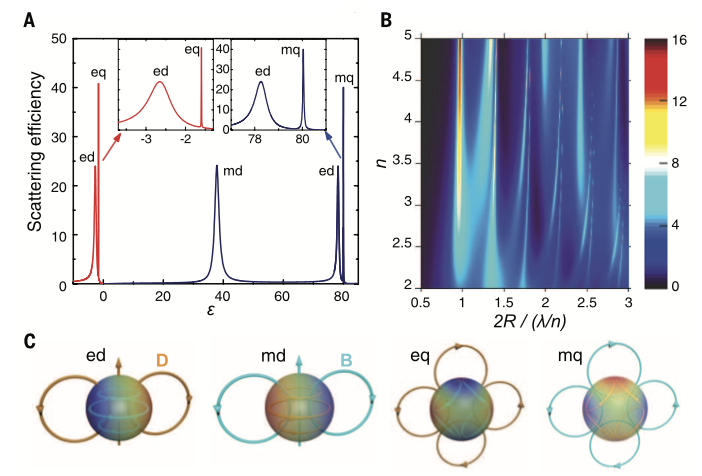
\includegraphics[width=0.7\linewidth]{images/fig1.png}
	\caption{Эффективность рассеяния (безразмерное отношение сечения рассеяния к геометрическому сечению частицы) в зависимости от диэлектрической проницаемости $\varepsilon$ (частицы без потерь, q = 0,5) для плазмонных ($\varepsilon$  < 0) и диэлектрических ( $\varepsilon$ > 0) материалов. Сокращения для резонансов: ed - электрический диполь; eq - электрический квадруполь; md - магнитный диполь; mq - магнитный квадруполь. (B) Эффективность рассеяния диэлектрической частицы без потерь (цветная шкала справа) как функция показателя преломления n и параметра размера. (C) Иллюстрация структур электрического и магнитного поля для различных электрических и магнитных резонансов, поддерживаемых сферической диэлектрической частицей.}
	\label{fig1}
\end{figure}
\hspace*{2mm}Чтобы проиллюстрировать фундаментальные свойства рассеяния света наночастицами, рассмотрим случай сферической частицы, освещенной плоской волной, для которой существует точное аналитическое решение уравнений Максвелла. Согласно теории Ми (3), металлические и диэлектрические сферические частицы могут обладать сильными резонансами рассеяния (рис. \ref{fig1}A). В случае безмасляных и немагнитных материалов их свойства рассеяния зависят только от двух параметров: диэлектрической проницаемости $\varepsilon$  и размерного параметра q, который пропорционален отношению радиуса наночастицы R к длине волны света $\lambda$ ($q = 2\pi R/\lambda$). Различие между металлическими и диэлектрическими частицами заключается в знаке диэлектрической проницаемости, которая является отрицательной для металлов и положительной для диэлектриков. Небольшие металлические сферы (q < 1) создают только локализованные поверхностные плазмонные резонансы электрического типа - дипольные, квадрупольные и т.д., в то время как их магнитный отклик остается практически незначительным из-за исчезающего поля внутри сферы (рис. \ref{fig1}А).  Чтобы создать магнитный отклик от металлических структур, геометрия частицы должна быть изменена. Например, резонатор с разрезным кольцом (4) работает аналогично эффективной LC-схеме (то есть, цепи индуктор-конденсатор) с усилением магнитного поля в центре. Для диэлектрических частиц мы можем наблюдать как электрический, так и магнитный отклики сравнимых сил (рис. \ref{fig1}А). Резонансный магнитно-дипольный отклик является результатом связи входящего света с круговыми токами смещения электрического поля вследствие проникновения поля и замедления фазы внутри частицы. Это происходит, когда длина волны внутри частицы становится сопоставимой с диаметром частицы $2R \approx \lambda/n$ (рис. \ref{fig1}В). Полевая структура четырех основных резонансных мод в диэлектрических частицах с высоким индексом - магнитном диполе, электрическом диполе, магнитном квадруполе и электрическом квадруполе - показана на рис. \ref{fig1}С. На длине волны магнитного резонанса возбужденная магнитно-дипольная мода диэлектрической сферы с высоким показателем может вносить основной вклад в эффективность рассеяния, превосходя таковую других мультиполей на порядки величины.
\\
\hspace*{2mm}
Из теории Ми следует, что максимально достижимая эффективность рассеяния для конкретного многополярного возбуждения субволновой частицы зависит только от резонансной частоты, а не от типа материала (5). Это говорит о том, что многие плазмонные эффекты, наблюдаемые при рассеянии света металлическими наночастицами, могут быть реализованы с помощью диэлектрических наночастиц с высоким индексом. На рисунке \ref{fig1}B показано масштабирование различных резонансов по отношению к показателю преломления n. При n > 2 все основные мультиполи хорошо определены, и их спектральные положения соответствуют фиксированному отношению длины волны внутри частицы к ее диаметру. Эффективность рассеяния всех мультиполей также увеличивается с ростом n (6–9).
\\
\hspace*{2mm}
Сильные оптически индуцированные магнитные дипольные резонансы в диэлектрических наночастицах с высоким индексом могут быть достигнуты не только для сфер, но и для сфероидов (10, 11), дисков и цилиндров (12), колец (13) и многих других геометрий (14). ). Это обеспечивает важные возможности для создания разнообразных полностью диэлектрических наноструктур с желаемыми спектральными положениями резонансов. Изменяя геометрические параметры частиц, спектральные положения как электрического, так и магнитного дипольного резонансов могут настраиваться независимо, чередуя или перекрывая друг друга на одной частоте для простых геометрий (11, 12, 15).


\subsection{Наблюдение оптических магнитных резонансов в диэлектрических наночастицах.}

Кремниевые (Si) наносферы с размерами от 100 до 300 нм поддерживают сильные магнитные и электрические дипольные резонансы в видимой и ближней ИК областях спектра (рис. \ref{fig2}). 
 \begin{figure}[h!]
	\centering
	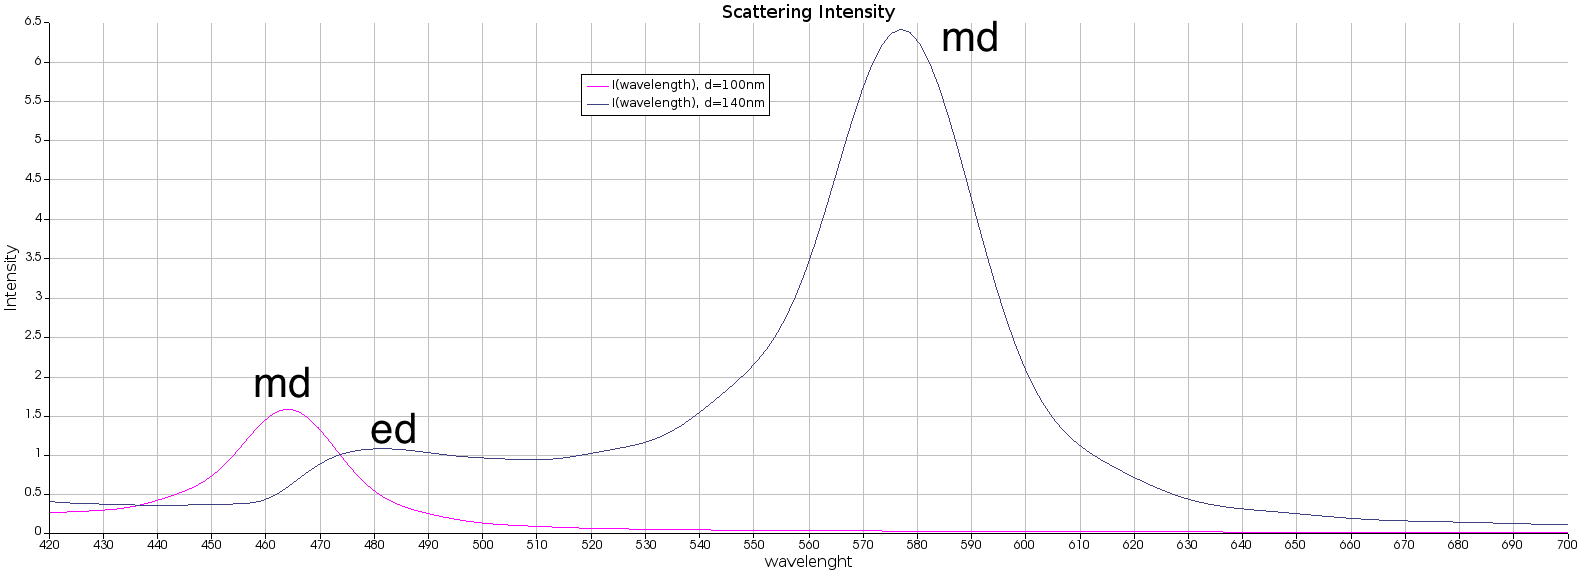
\includegraphics[width=0.7\linewidth]{images/graph1.png}
	\caption{Результат моделирования оптического магнитного отклика наночастиц кремния  диаметром 100 нм. (розовый график) и 140 нм. (синий график).  Сокращения для резонансов: ed - электрический диполь; md - магнитный диполь}
	\label{fig2}
\end{figure}
Экспериментальная демонстрация электрических и магнитных дипольных резонансов на видимых длинах волн впервые была представлена для сферических наночастиц Si, полученных с помощью фемтосекундной лазерной абляции на кремниевых и стеклянных подложках (8, 20). 
 \begin{figure}[h!]
	\centering
	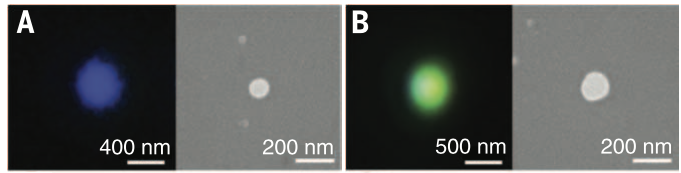
\includegraphics[width=0.7\linewidth]{images/fig2.png}
	\caption{ Изображения в темнопольном оптическом микроскопе (слева), изображения на сканирующем электронном микроскопе (SEM) (справа)  сферических наночастиц Si с приблизительными диаметрами 100 нм (A) 140 нм (В)  (8)}
	\label{fig3}
\end{figure}
\hspace*{2mm}Различные цвета, наблюдаемые на темнопольных микроскопах (рис. \ref{fig3}), соответствуют магнитным дипольным резонансам почти идеальных сферических наночастиц Si с размерами от 100 до 200 нм (8).  Помимо кремния, полупроводники группы IV и группы III-V с показателями преломления выше 2 могут иметь аналогичные оптические свойства в зависимости от их поглощения и показателя преломления в конкретном диапазоне длин волн. Например, магнитные и электрические дипольные резонансы недавно были экспериментально обнаружены в нанодисках арсенида галлия (GaAs) в видимом спектре (26) и теллура (Te) в среднем ИК-спектре (27).



\section{Нелинейная оптика с резонансными диэлектрическими наноструктурами}
\hspace*{2mm}Усиление в ближнем поле электрического и магнитного отклика в полностью диэлектрических наноструктурах может привести к новым нелинейным эффектам. В частности, генерация второй и третьей гармоник (SGH и THG), самоиндукция света и комбинационное рассеяние подвержены сильному ограничению в результате геометрических резонансов. Известно, что плазмонные резонансы, которые усиливают локальные электрические поля, усиливают нелинейно-оптические эффекты в металлических наноструктурах. В отличие от плазмоники, резонансы диэлектрических наночастиц с высоким индексом обеспечивают модовый объем, который не ограничивается интерфейсами и, следовательно, может привести к более высокой эффективности преобразования.


\subsection{Генерация третьей гармоники в наночастицах кремния, обусловленная магнитным откликом}
\hspace*{2mm}Усиленная THG от нанодисков Si, демонстрирующих как электрический, так и магнитный дипольный резонансы, наблюдалась экспериментально (58) с помощью микроскопии и спектроскопии третьей гармоники, причем сигнал TH усиливался вблизи магнитного дипольного резонанса. Сканирующая электронная микрофотография нанодисков показана на рисунке $\ref{nonliner:nanodisks1}$а. На рисунке $\ref{nonliner:nanodisks1}$b показан отрицательный логарифм спектра пропускания, полученный для этого образца с использованием установки, основанной на источнике белого света и ИК-спектрометре. Спектр нормализован по спектру смежной области образца, где верхний слой Si вытравлен. 
\\
\hspace*{2mm}
Диски освещались интенсивным фемтосекундным лазерным импульсом с частотой $\omega$, близкой к магнитно-дипольному резонансу первого. В результате высокой восприимчивости кремния третьего порядка $\chi^3$ передаваемый сигнал содержал импульсы утроенной основной частоты $3\omega$. Поскольку сигнал третьей гармоники (TH) пропорционален кубу локальной напряженности поля, разумно ожидать значительного усиления процесса TH в нанодисках с их магнитными резонансами, возбуждаемыми фундаментальной волной. (рис. \ref{nonliner:nanodisks}). 
  \begin{figure}[h!]
	\centering
	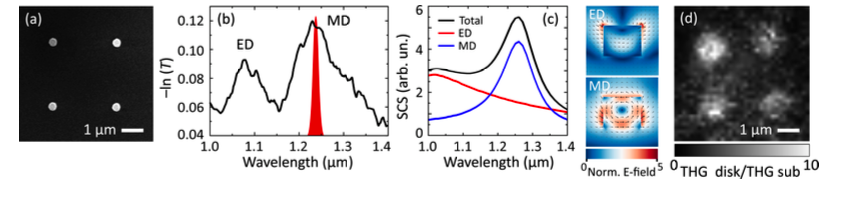
\includegraphics[width=1\linewidth]{images/fig4.png}
	\caption{Пространственно разделенные THG от отдельных нанодисков Si, усиленных магнитным резонансом. (а) Сканирующая электронная микроскопия изображения матрицы кремниевых нанодисков с d = 360 нм, h = 260 нм и p = 2,85 мкм. (b) Экспериментальный нормированный спектр пропускания образца (черный) со спектром импульса накачки, обозначенным красной областью. ED обозначает положение электрического дипольного резонанса, а MD обозначает положение магнитного дипольного резонанса. (c) Рассчитанные спектры сечения рассеяния (SCS) нанодисков (черный), разложенных на электрические дипольные (красные) и магнитные дипольные (синие) вклады с соответствующими распределениями электрического поля. (d) Микроскопическое изображение образца, полученное с помощью сканирующего оптического микроскопа путем обнаружения сигнала THG при $\lambda$ = 413 ± 5 нм. Сигнал нормализуется сигналом, полученным при тех же условиях из области подложки. THG с усилением локального поля наблюдается на участках нанодисков по сравнению с подложкой между ними.}
	\label{nonliner:nanodisks1}
\end{figure}
 \begin{figure}[h!]
	\centering
	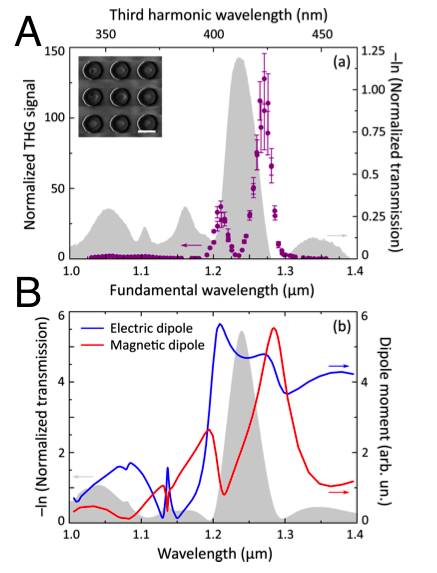
\includegraphics[width=0.5\linewidth]{images/fig3.png}
	\caption{(А). THG-спектроскопия массивов нанодисков Si. Отрицательный логарифм нормированного спектра пропускания образца с p = 0,8 мкм, h = 220 нм и d = 0,5 мкм дан с серой областью, указывающей на резонанс при 1,24 мкм. Спектр THG образца, нормированный по спектру подложки, показан фиолетовыми точками, который сильно усиливается в пределах спектральной полосы резонанса. На вставке показано SEM-изображение фрагмента образца. Масштабная линейка составляет 500 нм. (B) Моделируемый спектр пропускания основной длины волны через дисковый массив и подложку, демонстрирующий хорошее согласие с наблюдаемой передачей в эксперименте. Наложенные синие и красные кривые дают величину электрических и магнитных дипольных моментов (соответственно), индуцированных в одном диске в моделировании передачи. Эти дипольные моменты демонстрируют, что электрические и магнитные резонансы являются любой стороной наблюдаемого резонанса пропускания. Двухпиковая структура каждого спектра дипольного момента вносит вклад в двухпиковый спектр THG в (A).}
	\label{nonliner:nanodisks}
\end{figure}
\hspace*{2mm}Локализация поля в магнитном резонансе приводит к увеличению интенсивности гармоник на два порядка по отношению к неструктурированному объемному Si, при этом эффективность преобразования ограничивается только двухфотонным поглощением в подложке (58). 
\\
\hspace*{2mm}
Сильные THG также наблюдались на метаповерхностях на основе Si (59). Комбинируя эффект Керра с высококачественным факторным резонансом в линейном спектре пропускания метазерна, авторы продемонстрировали эффективность преобразования THG в $1,18\cdot 10^{-6}$ при пиковой интенсивности накачки 2 3,2 ГВт / см. Это соответствует yсилению сигнала THG в $1,5\cdot10^5$  по сравнению с  неструктурированной пленки Si с такой-же толщина. Недавние демонстрации также включить усиление THG в резонансных нанопиллярах изготовленного из высокоиндексных нецентросимметричных полупроводников III-V рода: GaAs (60) или AlGaAs (61). Коэффициент усиления $10^4$ по сравнению с неструктурированной GaAs пленкой показаны с полной эффективностью преобразования $2\cdot10^{-5}$  при интенсивности накачки 3,4 ГВт / см.Сильные квадратичные нелинейные процессы являются причиной усиления генерации запутанных фотонных пар посредством спонтанного параметрического преобразования с понижением частоты (SPDC) с диэлектрическими нанорезонаторами и экспериментальной реализации наноразмерных квантово-запутанных источников света, которые используют оптическую нелинейность.
\\
\hspace*{2mm}
Помимо генерации гармоник, была продемонстрирована эффективная настройка оптических свойств высокоиндексных наночастиц вблизи магнитных резонансов Ми-типа с помощью фемтосекундного лазерного излучения (62). Эффект основан на сверхбыстрой (<100 фс) фотоинжекции плотной электронно-дырочной плазмы внутри таких наночастиц, резко изменяя их переходную диэлектрическую проницаемость. Увеличение отражательной способности материала было порядка 20\%. В аналогичном эксперименте было показано сверхбыстрое полностью оптическое переключение в субволновых нелинейных диэлектрических наноструктурах с локальными магнитными резонансами (63). Измерения зонда накачки показали, что переключение в нанодисках может регулироваться ограниченным импульсом двухфотонным поглощением 65 фс, которое увеличивается в 80 раз по сравнению с неструктурированной кремниевой пленкой (63).
\\
\hspace*{2mm}
Эти экспериментальные демонстрации показывают большие перспективы для быстро развивающейся области нелинейной и квантовой нанофотоники. Основным преимуществом резонансных диэлектрических наноструктур перед плазмониками является локализация и сильное усиление оптических полей внутри частиц, что способствует сильным объемным нелинейностям и позволяет добиться высокой эффективности преобразования.

\section{Эффекты, связанные c поляризацией второго порядка}
\hspace*{2mm}Пусть на квадратично-нелинейную среду воздействует монохроматическое поле с частотой $\omega$:
 \begin{equation}\label{shg:e(t)}
A(t) = A\cos(\omega t)
\end{equation}
Тогда нелинейная поляризация второго порядка будет пропорциональна
полю во второй степени:

 \begin{equation}\label{shg:polarization}
P(t)^{(2)} = \chi^{(1)}E(t)^2 = \frac{1}{2}\chi^{(1)}A^2 + \frac{1}{2}\chi^{(1)}A^2\cos(2\omega t)
\end{equation}
Это значит, что поляризация будет иметь постоянную составляющую $ \frac{1}{2}\chi^{(1)}A^2$ , и
переменную $\frac{1}{2}\chi^{(1)}A^2\cos(2\omega t)$, на удвоенной частоте $2\omega$. Первое слагаемое в ($\ref{shg:polarization}$) соответствует нелинейному процессу, который называется оптическим выпрямлением, а второе – генерации второй гармоники



\subsection*{Возбуждение второй гармоники с использованием нарушенной симметрии III - V полупроводниковых метаповерхностей Фано}

\section{Эффекты, связанные c поляризацией третьего порядка}


\section{Эффекты связанные с поляризацией более выскоих порядков}


